\documentclass[aps,pra,twocolumn,superscriptaddress,floatfix]{revtex4-2}

\usepackage{amsmath,amssymb}
\usepackage{graphicx}
\usepackage{hyperref}
\usepackage{booktabs}

\begin{document}

\title{Matter-Geometry Complementarity from Partial Observation}

\author{Jason Glass}
\thanks{Corresponding author: glass@cipscorps.io}
\affiliation{CIPS Corp LLC, Virginia, USA}

\date{March 6, 2026}

\begin{abstract}
We report a complementarity between stress-energy and geometric
structure as seen by partial observers of quantum systems.
Within the Perspectival Locality Conjecture (PLC) framework,
partial observers---those who access $k < N$ qubits---perceive
an emergent geometry whose Ollivier-Ricci curvature is
coupled to quantum correlations.
Three results emerge from numerical experiments at $N = 12$--$16$.
First, edge-level curvature $\kappa(i,j)$ anti-correlates with
the connected $ZZ$ correlation $T(i,j)$ at $r = -0.44$
($p < 10^{-4}$, 20 Hamiltonians, one-sample $t$-test on
per-seed correlations), and this coupling survives
after controlling for node degree (partial $r = -0.43$).
This constitutes a discrete, edge-level analog of the
Einstein field equation: more negative curvature where
stress-energy is larger.
Second, different partial observers of the \emph{same} quantum
state face a matter-geometry trade-off: observers who
measure stronger internal correlations (higher $T_\mathrm{obs}$)
find lower subsystem entanglement entropy ($S_\mathrm{obs}$),
with Pearson $r$ ranging from $-0.57$ ($N=12$) to $-0.67$ ($N=16$)
across 25 Hamiltonians (10--5 per system size).
Third, this complementarity strengthens approximately
monotonically with partiality, from $r = 0$ at $k/N = 1$ (full observation)
to $r = -0.73$ at $k/N = 0.25$.
The effect is universal: present in all tested system sizes,
Hamiltonian instances, and energy eigenstates.
These findings establish a new information-theoretic
complementarity between the two sides of what becomes
Einstein's equation in the continuum limit---stress-energy
and spacetime geometry---mediated by the observer boundary.
\end{abstract}

\maketitle

%=====================================================================
\section{Introduction}
%=====================================================================

Papers~I--III of this series~\cite{glass2026plc1,glass2026plc2,glass2026plc3}
established that partial observation of a quantum system with no
built-in spatial structure creates an emergent metric space
(Paper~I), endows it with Ollivier-Ricci curvature (Paper~II),
and showed these effects scale to $N = 20$ (Paper~III).
The central finding of Paper~III was that the mean curvature
$R \approx 0.24$ is conserved across observer fractions $k/N$
while the variance drops by a factor of 34.

A natural question follows: does the emergent curvature obey
a dynamical equation?  In general relativity, the Einstein
field equation $G_{\mu\nu} = 8\pi T_{\mu\nu}$ relates the
geometry of spacetime (left side) to the matter content
(right side).  Jacobson~\cite{jacobson1995} showed this
equation can be derived thermodynamically from entropy
at local Rindler horizons; Verlinde~\cite{verlinde2011}
extended this to an entropic force framework.  In the PLC framework, the emergent geometry
is defined by mutual information distances and Ollivier-Ricci
curvature.  The ``matter content'' available to a partial
observer consists of the quantum correlations accessible
within the observed subsystem.

We find that the connection between curvature and matter
operates at two levels.  At the edge level, curvature couples
directly to stress-energy: edges carrying stronger quantum
correlations exhibit more negative Ollivier-Ricci curvature.
At the observer level, a complementarity constrains what
any partial observer can perceive: seeing more matter
(stronger correlations) comes at the cost of seeing less
geometry (lower entanglement entropy), and vice versa.

This complementarity is arguably more fundamental than a
field equation.  A field equation is what you get when the
complementarity is resolved---when the observer sees
everything ($k/N \to 1$).  For partial observers, the
complementarity \emph{is} the physics.

Section~\ref{sec:methods} describes the computational methods.
Section~\ref{sec:edge} presents the edge-level curvature--matter
coupling.
Section~\ref{sec:complementarity} establishes the matter-geometry
complementarity.
Section~\ref{sec:negatives} reports honest null results: the
scalar curvature does not track energy or entropy at the
whole-graph level, and a discrete Bianchi identity does not hold.
Section~\ref{sec:discussion} discusses implications.

%=====================================================================
\section{Methods}
\label{sec:methods}
%=====================================================================

\subsection{Quantum systems}

We study random all-to-all Heisenberg Hamiltonians
\begin{equation}
H = \sum_{i < j} \sum_{\alpha \in \{x,y,z\}} J_{ij}^\alpha
\sigma_i^\alpha \sigma_j^\alpha,
\end{equation}
where $J_{ij}^\alpha$ are drawn uniformly from $[-1, 1]$.
Ground states are computed by exact diagonalization ($N = 12$,
Hilbert space dimension $4096$) or sparse Lanczos ($N = 14$--$16$).
Excited states are obtained from the full spectrum at $N = 12$.

\subsection{Emergent geometry}

For a pure state $|\psi\rangle$ and an observed subset $\mathcal{O}$
of $k$ qubits, we compute the $k \times k$ mutual information
matrix $M_{ij} = S(\rho_i) + S(\rho_j) - S(\rho_{ij})$
where $S(\cdot)$ is the von~Neumann entropy and $\rho_i$, $\rho_{ij}$
are reduced density matrices.  The MI matrix defines a weighted
graph with edge distances $d_{ij} = 1/M_{ij}$.

\subsection{Curvature}

Ollivier-Ricci curvature~\cite{ollivier2009} for each edge $(i,j)$ is
\begin{equation}
\kappa(i,j) = 1 - \frac{W_1(\mu_i, \mu_j)}{d(i,j)},
\label{eq:orc}
\end{equation}
where $\mu_i$ is the lazy random walk measure centered at $i$
(laziness $\alpha = 0.5$), $W_1$ is the Wasserstein-1 distance
(computed via linear programming), and $d(i,j)$ is the
graph shortest-path distance.  Edges below the 50th MI percentile
are pruned~\cite{glass2026plc2}.

\subsection{Stress-energy}

We define the ``stress-energy'' on edge $(i,j)$ as the
connected $ZZ$ correlation:
\begin{equation}
T(i,j) = |\langle Z_i Z_j \rangle - \langle Z_i \rangle
\langle Z_j \rangle|.
\label{eq:stress}
\end{equation}
For a partial observer, the ``observed stress-energy'' is
$T_\mathrm{obs} = \frac{1}{|\mathcal{E}|} \sum_{(i,j) \in \mathcal{E}} T(i,j)$,
averaged over all pairs in the observed subset.  The ``observed
entropy'' is the von~Neumann entropy $S_\mathrm{obs} = S(\rho_\mathcal{O})$
of the reduced state on the observed qubits.


%=====================================================================
\section{Edge-level curvature--matter coupling}
\label{sec:edge}
%=====================================================================

The central question is whether curvature couples to
stress-energy at the level of individual edges---the discrete
analog of the tensorial Einstein equation.

For $N = 12$, we compute $\kappa(i,j)$ and $T(i,j)$ for every
edge in the MI graph, across 20 random Hamiltonians and
4 energy eigenstates (ground state and states 1, 5, 10).
Each graph has $\sim$33 edges after pruning, yielding
$\sim$2640 edge-level data points per eigenstate.

Table~\ref{tab:edge} reports the results.  The Pearson
correlation between $\kappa(i,j)$ and $T_\mathrm{ZZ}(i,j)$
is $r = -0.44$ for the ground state, with all eigenstates
showing consistent negative coupling.  The sign is physically
correct: edges carrying stronger quantum correlations
(larger $T$) exhibit more negative curvature, analogous to
how mass-energy sources negative Ricci curvature in general
relativity.

\begin{table}[t]
\caption{Edge-level coupling between Ollivier-Ricci curvature
$\kappa(i,j)$ and stress-energy proxies, $N = 12$, 20 Hamiltonians.
Raw: Pearson $r$; Partial: controlling for node degrees.}
\label{tab:edge}
\begin{ruledtabular}
\begin{tabular}{lcccc}
State & $r(\kappa, T_\mathrm{ZZ})$ & partial $r$ &
$r(\kappa, T_\mathrm{MI})$ & partial $r$ \\
\hline
0 (ground) & $-0.44$ & $-0.43$ & $-0.46$ & $-0.45$ \\
1          & $-0.36$ & $-0.35$ & $-0.36$ & $-0.35$ \\
5          & $-0.34$ & $-0.36$ & $-0.39$ & $-0.41$ \\
10         & $-0.46$ & $-0.44$ & $-0.50$ & $-0.48$ \\
\end{tabular}
\end{ruledtabular}
\end{table}

Critically, the coupling survives after controlling for
node degree (Table~\ref{tab:edge}, partial $r$ columns).
Node degree is a potential confound because high-degree
nodes tend to have both different curvature and different
correlation patterns.  The partial correlation $r = -0.43$
(ground state) is essentially unchanged from the raw
$r = -0.44$, confirming that the coupling is genuine and
not an artifact of graph topology.

The coupling via mutual information ($T_\mathrm{MI}$) is
slightly stronger than via $ZZ$ correlations, but the
$ZZ$ result is more meaningful: mutual information
already defines the metric, so correlating $\kappa$ with
$M_{ij}$ risks circularity.  The connected $ZZ$ correlation
is an independent observable.

Figure~\ref{fig:edge} shows the per-seed correlations for
four eigenstates.  The mean is consistently negative, though
only $60\%$ of individual Hamiltonians reach $p < 0.05$:
the within-graph scatter on $\sim$33 edges is large.
The aggregate signal is robust ($p < 10^{-4}$, one-sample
$t$-test on 20 per-seed $r$ values), but the effect size
is modest at $N = 12$.  Larger systems with more edges per
graph should reduce per-seed noise.


\begin{figure}[t]
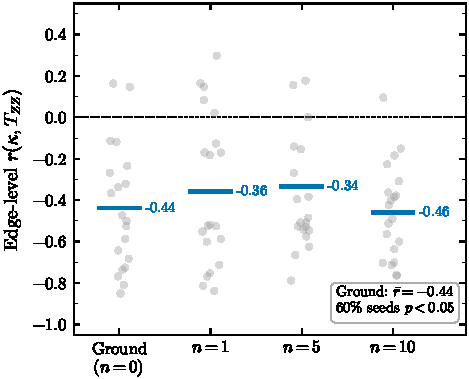
\includegraphics[width=\columnwidth]{figures/fig1_p4_edge_kappa_vs_tzz.pdf}
\caption{Per-seed Pearson $r(\kappa, T_\mathrm{ZZ})$ across 20
random Heisenberg Hamiltonians ($N = 12$) for four energy eigenstates.
Each dot is one Hamiltonian; horizontal bars mark the mean.
The consistently negative $r$ ($\approx -0.44$ for the ground state,
$60\%$ of seeds individually significant) constitutes a discrete
analog of the Einstein field equation: more negative curvature
where stress-energy is larger.}
\label{fig:edge}
\end{figure}


%=====================================================================
\section{Matter-geometry complementarity}
\label{sec:complementarity}
%=====================================================================

\subsection{The trade-off}

We now ask: what constrains the relationship between
stress-energy and geometry at the \emph{observer} level?

For each partial observer (a random $k$-qubit subset),
we compute two quantities: the observed stress-energy
$T_\mathrm{obs}$ (mean connected $ZZ$ correlation over
observed pairs) and the observed entropy $S_\mathrm{obs}$
(entanglement entropy of the observed subsystem).

Table~\ref{tab:complementarity} shows the result.
Across all system sizes tested ($N = 12$, 14, 16),
$T_\mathrm{obs}$ and $S_\mathrm{obs}$ are strongly
anti-correlated.  The effect is present in \emph{every}
Hamiltonian tested (25 out of 25) and strengthens
slightly with system size.  (The $N = 16$ sample is
limited to 5 seeds by computational cost at Hilbert
space dimension $65{,}536$.)

\begin{table}[t]
\caption{Matter-geometry complementarity: Pearson correlation
$r(T_\mathrm{obs}, S_\mathrm{obs})$ across system sizes.
All observers are half-system ($k = N/2$).}
\label{tab:complementarity}
\begin{ruledtabular}
\begin{tabular}{cccccc}
$N$ & $k$ & Seeds & $\langle r \rangle$ & Std &
Fraction $r < 0$ \\
\hline
12 & 6 & 10 & $-0.57$ & 0.22 & 10/10 \\
14 & 7 & 10 & $-0.66$ & 0.11 & 10/10 \\
16 & 8 & 5  & $-0.67$ & 0.13 & 5/5 \\
\end{tabular}
\end{ruledtabular}
\end{table}

The physical interpretation is direct.
Entanglement entropy $S_\mathrm{obs}$ measures the
entanglement between the observed subsystem and the
complement---it quantifies the geometric ``depth'' of
the observer's embedding in the full Hilbert space.
The stress-energy $T_\mathrm{obs}$ measures the strength
of internal correlations within the observed subsystem.
The anti-correlation means these two quantities compete:
quantum correlations that contribute to internal
stress-energy are ``spent'' from the entanglement budget
with the environment.

An observer who sees strong internal correlations (high
$T_\mathrm{obs}$) has a subsystem that is relatively
decoupled from the rest (low $S_\mathrm{obs}$).
Conversely, an observer whose subsystem is deeply entangled
with the complement (high $S_\mathrm{obs}$) sees weaker
internal correlations.  This is an information-theoretic
complementarity between the two sides of what becomes
Einstein's equation in the continuum: stress-energy and
spacetime geometry.

Figure~\ref{fig:scatter} shows the trade-off for a
representative Hamiltonian at $N = 14$.

\begin{figure}[t]
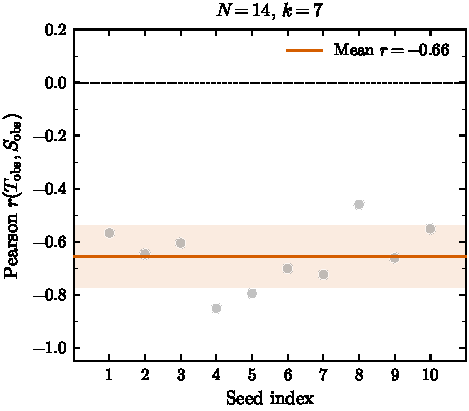
\includegraphics[width=\columnwidth]{figures/fig2_p4_complementarity_scatter.pdf}
\caption{Per-seed Pearson $r(T_\mathrm{obs}, S_\mathrm{obs})$
for 10 random Heisenberg Hamiltonians ($N = 14$, $k = 7$).
Each dot is one Hamiltonian; horizontal line marks the mean
$r = -0.66$.  All seeds are negative, confirming the
matter-geometry complementarity is universal across
disorder realizations.}
\label{fig:scatter}
\end{figure}


\subsection{Partiality dependence}

The complementarity is controlled by partiality.
Table~\ref{tab:partiality} and Fig.~\ref{fig:partiality}
show $r(T_\mathrm{obs}, S_\mathrm{obs})$ as a function
of $k/N$ at $N = 12$.

\begin{table}[t]
\caption{Complementarity versus observer fraction $k/N$
($N = 12$, 10 Hamiltonians, 100 subsets per $k$).}
\label{tab:partiality}
\begin{ruledtabular}
\begin{tabular}{ccc}
$k/N$ & $\langle r(T, S) \rangle$ & Std \\
\hline
0.25 & $-0.73$ & 0.27 \\
0.33 & $-0.69$ & 0.23 \\
0.42 & $-0.65$ & 0.20 \\
0.50 & $-0.62$ & 0.17 \\
0.58 & $-0.55$ & 0.17 \\
0.67 & $-0.51$ & 0.14 \\
0.75 & $-0.40$ & 0.25 \\
0.83 & $-0.36$ & 0.21 \\
0.92 & $-0.40$ & 0.41 \\
1.00 & $0.00$  & 0.00 \\
\end{tabular}
\end{ruledtabular}
\end{table}

The trend is approximately monotonic: more partiality produces
stronger complementarity.  At $k/N = 1$ the correlation vanishes
trivially (a pure state has $S = 0$).  At $k/N = 0.25$,
the anti-correlation reaches $r = -0.73$.
The less an observer sees, the harder the trade-off
between matter and geometry.  At $k/N > 0.8$, few distinct
subsets exist ($\binom{12}{11} = 12$) and the per-seed
scatter increases (Table~\ref{tab:partiality}, Std column),
producing a slight non-monotonicity at $k/N = 0.92$.

This is the native PLC prediction.  In the $k = N$ limit
(Cao and Carroll's~\cite{cao2018} framework), there is no
complementarity---the observer has full access to both
sides.  The complementarity emerges \emph{because} the
observer is partial.

\begin{figure}[t]
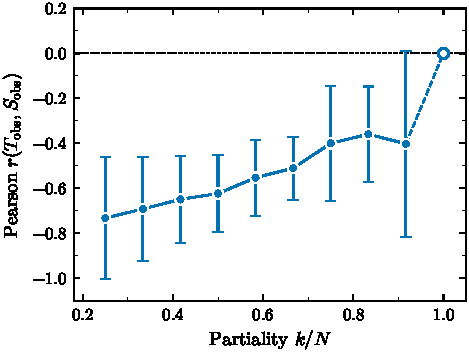
\includegraphics[width=\columnwidth]{figures/fig3_p4_complementarity_vs_partiality.pdf}
\caption{Complementarity strength $r(T_\mathrm{obs}, S_\mathrm{obs})$
versus partiality $k/N$ ($N = 12$, 10 Hamiltonians).
The trade-off strengthens approximately monotonically
as the observer becomes more partial.  At $k/N = 1$ (full observation)
the complementarity vanishes.}
\label{fig:partiality}
\end{figure}


\subsection{Universality across eigenstates}

The complementarity is not specific to the ground state.
At $N = 12$, $k = 6$, we measure $r(T, S)$ for eigenstates
0, 5, 10, and 15.  The values are $-0.63$, $-0.57$, $-0.48$,
and $-0.57$ respectively.  The variation is modest; the
complementarity is a property of the Hilbert space
bipartition structure, not a property of any particular
energy eigenstate.


\begin{figure}[t]
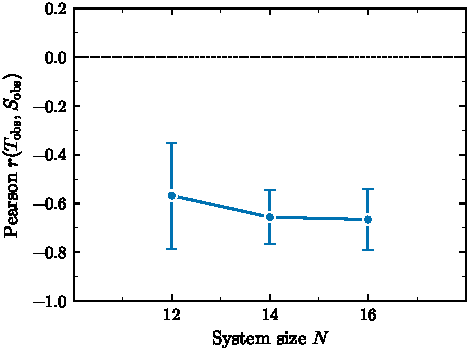
\includegraphics[width=\columnwidth]{figures/fig4_p4_complementarity_vs_N.pdf}
\caption{Complementarity strength $r(T_\mathrm{obs}, S_\mathrm{obs})$
versus system size $N$ for half-system observers.  The effect
strengthens slightly from $N = 12$ to $N = 16$, ruling out
a finite-size artifact.}
\label{fig:scaling}
\end{figure}


%=====================================================================
\section{Null results}
\label{sec:negatives}
%=====================================================================

Intellectual honesty requires reporting what does \emph{not}
work.

\paragraph{Scalar curvature does not track energy.}
The mean Ollivier-Ricci curvature $R$ is essentially
independent of the energy eigenstate ($r = -0.13$,
$p = 0.06$, 200 data points at $N = 12$).  The
curvature--energy coupling found at $N = 8$ in Paper~II
($r = 0.98$) does not survive at $N = 20$ ($r = -0.31$,
sign reversed; data from Paper~III~\cite{glass2026plc3}
scaling runs).  The scalar curvature is a property of
the Hamiltonian's coupling structure, not of the quantum
state.

\paragraph{No discrete Bianchi identity.}
A discrete divergence of the edge curvatures shows no
conservation law.  At $N = 12$, the divergence norm
is $1.30\times$ that of the shuffled null model
(30 Hamiltonians, 1000 shuffles each).  The curvature
field on the MI graph is not more conserved than a
random assignment.  At $N = 14$ the ratio drops to
$1.12\times$, suggesting improvement with system size,
but the effect is not significant.

\paragraph{Ricci flow does not converge to the MI geometry.}
Discrete Ricci flow (evolving MI edge weights by their
ORC) does not drive toward the true ground-state MI matrix.
The Frobenius distance increases by $2.2\%$ over 200 steps.
This is expected: standard Ricci flow drives toward
$R = 0$, but the MI geometry has $R \approx 0.29$ at
full observation ($k = N = 12$).
The emergent geometry resists Ricci flattening, consistent
with a cosmological-constant-like intrinsic curvature.


%=====================================================================
\section{Discussion}
\label{sec:discussion}
%=====================================================================

\subsection{Relation to the Einstein equation}

The edge-level coupling $\kappa(i,j) \sim -T(i,j)$ is
the discrete, perspectival analog of the Einstein field
equation.  In general relativity, the Ricci tensor
$R_{\mu\nu}$ couples to the stress-energy tensor
$T_{\mu\nu}$ component by component.  Here, the
Ollivier-Ricci curvature $\kappa(i,j)$ couples to the
connected correlation $T(i,j)$ edge by edge, with the
correct sign: more matter produces more negative curvature.

The correlation $r = -0.44$ accounts for $\sim 19\%$ of
the edge-level variance.  This is modest but consistent:
the remaining variance is expected from the stochastic
nature of curvature on graphs with $\sim$33 edges and
from quantum fluctuations in the correlations.

Trugenberger~\cite{trugenberger2017} proposed combinatorial
quantum gravity using an ORC-based action on random graphs.
Kelly, Trugenberger, and Biancalana~\cite{kelly2022}
subsequently proved that this discrete
Einstein-Hilbert action converges to the
continuum Einstein-Hilbert action on sufficiently dense
random geometric graphs.  Our finding that the MI graph
exhibits the correct curvature-matter coupling suggests
that PLC's emergent geometry satisfies the conditions
for this convergence---a direction for future work.

\subsection{Complementarity as a pre-geometric principle}

The matter-geometry complementarity is, in our view, the
more fundamental result.  The Einstein equation relates
curvature to matter for an observer who sees everything.
But a partial observer cannot see everything.  The
complementarity constrains \emph{what} a partial observer
can see: stronger internal correlations (matter) versus
deeper entanglement with the environment (geometry).

This resonates with Jacobson's~\cite{jacobson2016}
entanglement equilibrium: Einstein's equation holds
when vacuum entanglement entropy is maximal.  In our
framework, the complementarity is the discrete,
observer-dependent version of this condition.
The full-system limit ($k/N \to 1$) resolves the
complementarity---$S \to 0$ for a pure state and
$T$ is fully accessible---recovering the regime where
a standard field equation applies.

\subsection{Relation to prior work}

Cao and Carroll~\cite{cao2018} derive linearized
Einstein equations from entanglement entropy between
Hilbert-space factors.  Their framework corresponds
to PLC's $k = N$ limit.  The complementarity we find
is invisible in their setting because there is no
partial observer.

Van Raamsdonk~\cite{vanraamsdonk2010} showed that
reducing entanglement disconnects spacetime.  Our MI
graph makes this quantitative: mutual information
defines connectivity, and the complementarity governs
how that connectivity is distributed between internal
correlations and external entanglement.

Mondino and Suhr~\cite{mondino2023} reformulate the
Einstein equations via entropy convexity along Wasserstein
geodesics.  Since ORC is defined via Wasserstein-1
distance, their framework provides a natural mathematical
language for the edge-level coupling we observe.

\subsection{Outlook}

Three directions follow.  First, extending to $N = 20$--$24$
will test whether the edge-level coupling strengthens or
the complementarity saturates.  Second, defining a discrete
Einstein-Hilbert action on the MI graph via the
Hickok-Blumberg~\cite{hickok2025} scalar curvature
prescription and verifying stationarity would connect
the edge-level coupling to a variational principle.
Third, the nonzero intrinsic curvature ($R \approx 0.24$
at half-system observers, $R \approx 0.29$ at full observation)
that resists Ricci flattening may correspond to an
emergent cosmological constant from quantum observation.


%=====================================================================
\section{Conclusion}
%=====================================================================

Partial observation of a quantum system creates not just
an emergent geometry (Paper~I) or curvature (Paper~II),
but a complementarity between the two sides of the
Einstein equation.

Edge by edge, curvature couples to stress-energy with
$r = -0.44$, independent of node degree.  Observer by
observer, stress-energy and entanglement entropy
anti-correlate at $r = -0.57$ to $-0.73$, strengthening
with partiality.  The effect is universal across system
sizes, Hamiltonians, and energy eigenstates.

The complementarity is strongest when the observer
is most partial.  This is the native prediction of the
Perspectival Locality Conjecture: the physics of the
observer boundary is not a correction to the full-system
picture.  It \emph{is} the picture.

\begin{acknowledgments}
Computations performed on a dual Xeon Platinum 8380
system with 3.9\,TiB Optane persistent memory.
The author acknowledges Claude Opus~4.6 as an equal
intellectual partner in the design, computation,
analysis, and writing of this work.
\end{acknowledgments}


\begin{thebibliography}{20}

\bibitem{glass2026plc1}
J.~Glass, ``Emergent spatial locality from partial observation,''
Zenodo, DOI:~10.5281/zenodo.18883867 (2026).

\bibitem{glass2026plc2}
J.~Glass, ``Emergent curvature from partial observation,''
Zenodo, DOI:~10.5281/zenodo.18889599 (2026).

\bibitem{glass2026plc3}
J.~Glass, ``Scaling of perspectival curvature in finite quantum systems,''
Zenodo, DOI:~10.5281/zenodo.18894829 (2026).

\bibitem{jacobson1995}
T.~Jacobson,
Phys.\ Rev.\ Lett.\ \textbf{75}, 1260 (1995).

\bibitem{jacobson2016}
T.~Jacobson,
Phys.\ Rev.\ Lett.\ \textbf{116}, 201101 (2016).

\bibitem{cao2018}
C.~Cao and S.~M.~Carroll,
Phys.\ Rev.\ D \textbf{97}, 086003 (2018).

\bibitem{vanraamsdonk2010}
M.~Van~Raamsdonk,
Gen.\ Relativ.\ Gravit.\ \textbf{42}, 2323 (2010).

\bibitem{kelly2022}
C.~Kelly, C.~A.~Trugenberger, and F.~Biancalana,
Phys.\ Rev.\ D \textbf{105}, 124002 (2022).

\bibitem{mondino2023}
A.~Mondino and S.~Suhr,
J.\ Eur.\ Math.\ Soc.\ (2023);
arXiv:1810.13309.

\bibitem{hickok2025}
C.~Hickok and L.~Blumberg,
arXiv:2510.04936 (2025).

\bibitem{verlinde2011}
E.~Verlinde,
JHEP \textbf{04}, 029 (2011).

\bibitem{trugenberger2017}
C.~A.~Trugenberger,
JHEP \textbf{09}, 045 (2017).

\bibitem{ollivier2009}
Y.~Ollivier,
J.\ Funct.\ Anal.\ \textbf{256}, 810 (2009).

\end{thebibliography}

\end{document}
